\documentclass[12pt,letterpaper]{book}
\usepackage{amsmath}
\usepackage[utf8]{inputenc}
\usepackage{graphicx}

\title{Existencia de la economia dual en Colombia}
\author{Augusto Rico}
\date{\today}

\graphicspath{{Fig/}}

\newcommand*{\captionsource}[2]{%
    \textbf{\\Tomado:} #2%
  }%


\begin{document}
\maketitle
\section{Introduccion}

\begin{flushleft}   


el siguiente articulo esta enfocado en comprobar empiricamente la existencia de una economia dual en Colombia tal como plantea Lewis(1954).
Esta hipotesis se basa en la consideracion por parte del FMI(2020) de Colombia como una economia en via de Desarrollo, por ende si esto es cierto 
y basandonos en la tesis de W.Arthur Lewis Colombia debe tener tambien las caracteristicas de una economia Dual.\\
~\\
las economias en via de desarrollo tal como plantea Lewis(1954) estan caracterizadas por la coexistencia de dos tipos de economia, la moderna caracterizada
por altos niveles relativos de productividad ya que son intensivas en bienes de capital, y la economia tradicional caracterizada por bajos niveles de productividad
debido no existencia de bienes de capital en este sector, lo que implica bajos salarios para los trabajadores.\\
~\\
En Colombia este hecho se puede ver reflejado principalmente en las diferencias economicas entre las ciudades principales y las zonas rurales, que como se expondra
las ciudades princiaples estan caracterizadas por tener sectores modernos e industriales con altos niveles relativos de ingresos y bienestar, y las zonas rurales
apartadas del centro caracterizadas por la escazes de bienes de capital y un fuerte sector rural con baja productividad sostenido por uso intensivo de mano de obra con salarios de subsitencia.\\
~\\
en el trabajo se evaluara la existencia de una economia dual en Colombia, mediante indicadores de ingersos, calidad de vida, capacidad productiva para comprender si
exite efectivamente las dos economias en colombia, para esto se evaluara los datos segun divisiones administrativas, ya que aunque puedan coexistir estas dos economias por ejemplo en bogota
se tiene datos insuficientes para poder evaluarlo a una escala inferior.\\

\end{flushleft}

\section{Contexto Geografico e Historico}

\begin{flushleft}

Los habitantes de las distintas regiones del pais han estado historicamente aislados por la complicada geografia del pais, esto ha generado una clara desigudalda en el desarrollo nacional
el cual ha estado marcado por bonanzas de materias primas, principalmente cafe y petroleo, que logro mejorar las condiciones economicas y productivas de las zonas donde eran explotados estos recursos, y el periodo de
Sustitucion de importaciones donde se inicio con el proceso de industrializacion pero focalizado unicamente en las ciudades principales generando claras diferencias entre la division centro-perisferia. (Hahn \& Mesiel, 2018) \\
~\\
Dada la naturaleza centralizta de colombia y tal como afirman Junguito \& Rincon (2004) con un aumento del gasto publico que paso en la primera mital del siglo XX del 5 a cerca del 10\% del PIB en 1990 impulso
 principalmente el desempeño economico de Bogota, que adicionalmente con el proceso de sustitucion de importaciones le genero un mayor impulso a la desigualdad entre centro y perisferia debido a que
 mientras las ciudades principales eran beneficiadas gracias a la industrializacion las regiones perisfericas que el gobierno central no se interezo en industrializar sufrian el aumento en los costes asociados de produccion lo que reduccia su capacidad de inversion
 y por ende una incapacidad de lograr aumentar su productividad.\\
~\\

\end{flushleft}

\section{Desigualdad de ingresos}

\begin{flushleft}

La caracterictica principal de un mercado con economia dual es la abrupta diferencia entre los empleados del sector moderno y tradicional ya que esto denota
la expansion heterogenea del capitalismo en una zona, esto se ve reflejado en colombia tal como planteaba Furtado(1959) con una dominacion-dependencia en las relaciones centro-perisferia nacionales
donde los altos ingresos se encuentran concentrados en las ciudades principales del pais con procesos capitalistas equiparables a paises desarrollados  mientras 
se tiene zonas perisfericas con procesos pseudofeudales intensivos en mano de obra por el desinteres del centro para desarrollar estas economias.\\ 
~\\
\begin{figure}
    \centering
    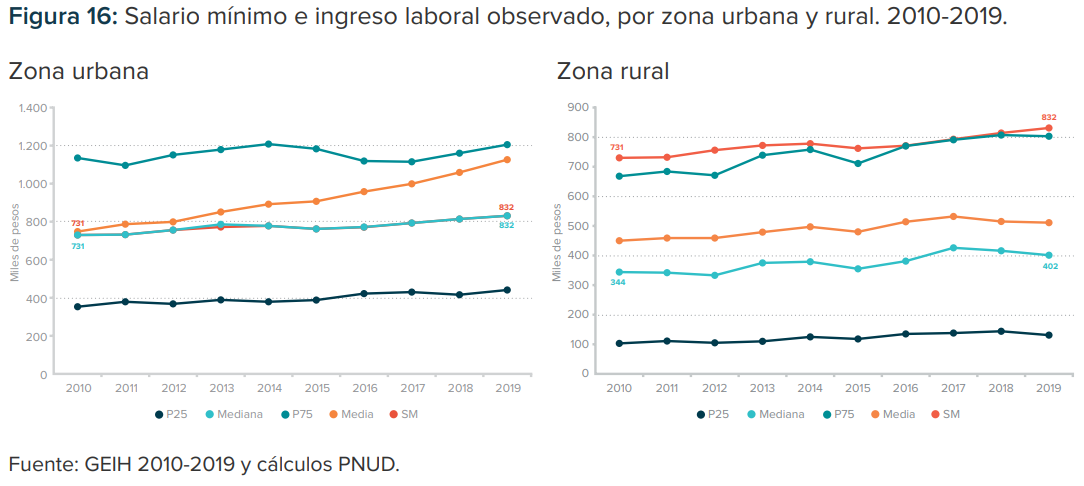
\includegraphics[width=\linewidth]{ingcentro-perisferia.png}
    \captionsource{Caption}{Mision de Empleo (2021)}
\end{figure}

Tal como se observa en las graficas en colombia existe una clara economia dual medida mediante los ingresos laborales, mientras en las zonas urbanas el salario minimo se ajusta a la mediana del salario,
en las zonas rurales en cambio el salario minimo no es siquiera superado por tres cuartas partes de los trabajadores rurales lo que evidencia una clara desigualdad en los ingresos entre estas dos economias.\\
~\\
\begin{figure}
    \centering
    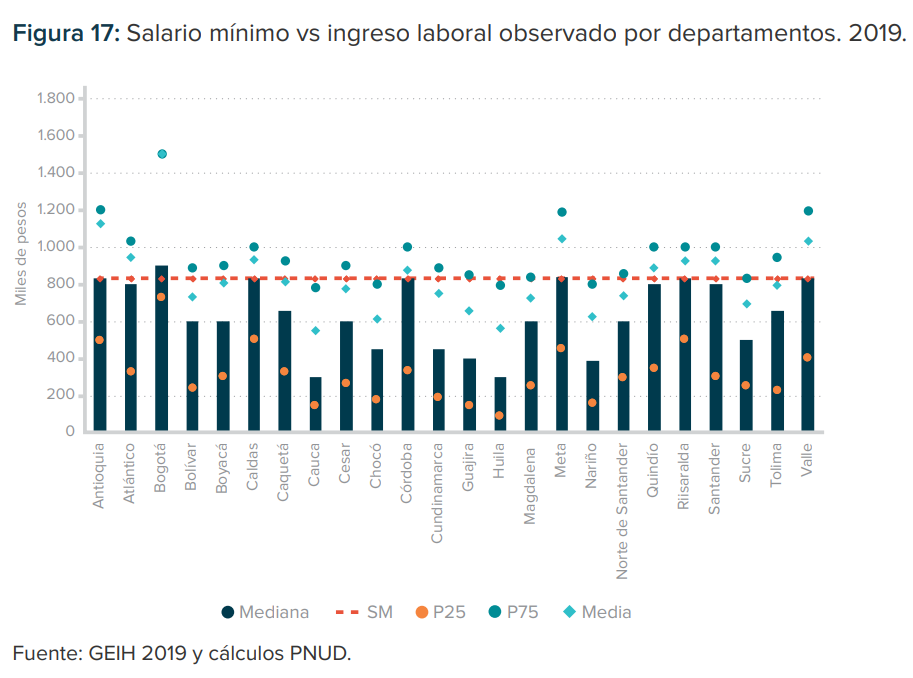
\includegraphics[width=\linewidth]{ingdepto.png}
    \captionsource{Caption}{Mision de Empleo (2021)}
\end{figure}

si este mismo analizis es realizado mediante la comparacion de ingresos en departamentos se obtiene mejores evidencias de la existencia de una economia dual en Colombia enmarcada en una fuerte dependencia
centro-perisferia donde la unica zona que logra que su mediana de salario supere el salario minimo es Bogota, la capital, y se le acercan zonas economicamente centrales tales como Atlantico, Antioquia, y Valle del Cauca u otras zonas que en algun punto
han experimentado bonanzas tales como la zona cafetera o petrolera.\\
\end{flushleft}

\section{Flujos Migratorios Internos}

\begin{flushleft}

Otra caracterictica de una economia dual es la absorcion de mano de obra proveniente del sector tradicional en el sector moderno, esto se puede 
ver reflejado en los flujos migratorios internos por departamentos perisfericos con economias tradicionales hacia economias modernas, esto sin ignorar el contexto de violencia que pueda existir en estas zonas.\\
~\\
\begin{figure}
    \centering
    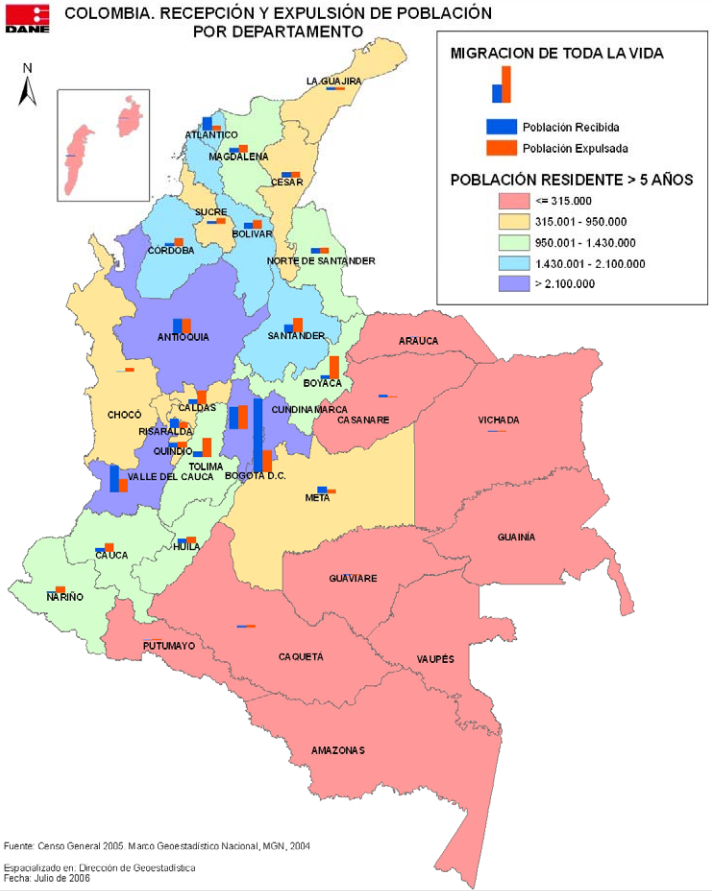
\includegraphics[width=10cm]{flujos.png}
    \captionsource{Caption}{Dane, Censo 2005}
\end{figure}

en concordancia con la teoria de la economia dual y lo expuesto anteriormente se puede observar que el mayor receptor neto de flujos migratorios internos
 es bogota y otras zonas centrales como Atlantico y Valle del Cauca, mientras que zonas que presentaban bajos niveles de ingresos tales como Cauca, Nariño o Boyaca son expulsores de poblacion, 
 por lo que se puede comprender que en Colombia esta existiendo una absorcion perfecta por parte del sector moderno tal como plantea la teoria.
\end{flushleft}

\end{document}